\subsection{Workflow Construction}

The workflow is constructed in four major stages.

\paragraph{Stage 1: phenotype cleaning.}
Phenotype processing is performed first because the task is defined by antibiotic-specific labels. Rows with missing key fields, ambiguous labels, or contradictory duplicates are removed. Only resistant and susceptible labels are kept for binary modeling. Antibiotics with too few records or too few resistant examples are excluded from the final cohort.

\paragraph{Stage 2: genotype cleaning.}
Genotype processing starts from determinant-level records. Exact duplicates are removed. If the same gene or mutation is detected multiple times in one isolate, only one preferred record is kept. Noisy categories are filtered out, and class and subclass labels are normalized so that later matching against antibiotic groups stays consistent.

\paragraph{Stage 3: genotype-to-phenotype connection.}
For each antibiotic, genotype rows are connected to phenotype labels under one of three scopes: \textit{strict}, \textit{broad}, or \textit{all}. This is the key design choice of the project because it controls how narrowly or broadly the features are selected before learning begins.

\begin{figure}[H]
\centering
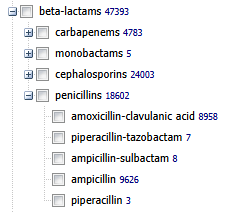
\includegraphics[width=0.45\textwidth]{figures/scope_broad_example}
\caption{Broad class hierarchy for beta-lactam antibiotics.}
\label{fig:broad-scope-example}
\end{figure}

\paragraph{Stage 4: model-ready table generation.}
After connection, the genotype evidence is converted into antibiotic-specific feature tables. These tables are the final inputs for XGBoost and for the rule-based baselines. Each table represents one modeling problem for one antibiotic under one biological scope, with one row per isolate.

\begin{figure}[H]
\centering
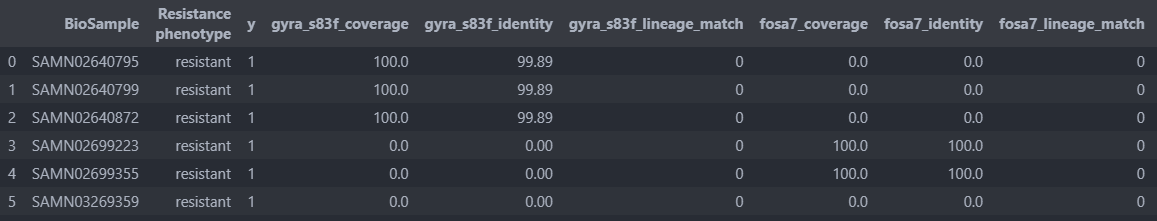
\includegraphics[width=0.9\textwidth]{figures/prepared_input_example}
\caption{Example of a prepared model-input table after genotype evidence has been aligned with phenotype labels.}
\label{fig:prepared-input-example}
\end{figure}

This staged construction separates data cleaning decisions from modeling decisions and makes each step easier to explain.
